\documentclass[11]{report}
\usepackage{graphicx}
\usepackage[a4paper]{geometry}
\usepackage{amsmath}
\usepackage{amssymb}
\usepackage{esint}
\usepackage{float}
\usepackage{hyperref}
\usepackage[utf8]{inputenc}
\usepackage[english]{babel}


\renewcommand{\baselinestretch}{1.2}
\geometry{margin=1in}
\pagenumbering{arabic}
\pagestyle{plain}
\begin{document}
\begin{titlepage}
\begin{center}
\vspace*{1cm}
\LARGE
\textbf{Documentation for Differential Forms Summer Project}\\
\vspace{5cm}
\normalsize
\textbf{Moustafa Gharamti, Samuel Kirwin-Jones, Maciej Tomasz Jarema}\\

\end{center}
\end{titlepage}

\section{Geometry of stack vectors}

\subsection{Translations needed to define stack vectors and arrowheads}
Stack vectors are covariant vectors, defined by planar sheets (lines, when working in 2D) perpendicular to arrows of the contravariant vector. The density of these planes, is determined by magnitude of the vector field at each point in space. These stack vectors, being covariant, correspond to differential forms, while arrow vectors (being contravariant) correspond to vector fields.\\
In python, these stack sheets have to be defined from the magnitude and direction of the input, based on \(x\) and \(y\) components of the 1-from.

\begin{figure}[H]
	\centering
	%\graphicspath{ {c:/Users/macus/Desktop/Uni/summer internships/Moustafa - Differential Forms/images/} }
	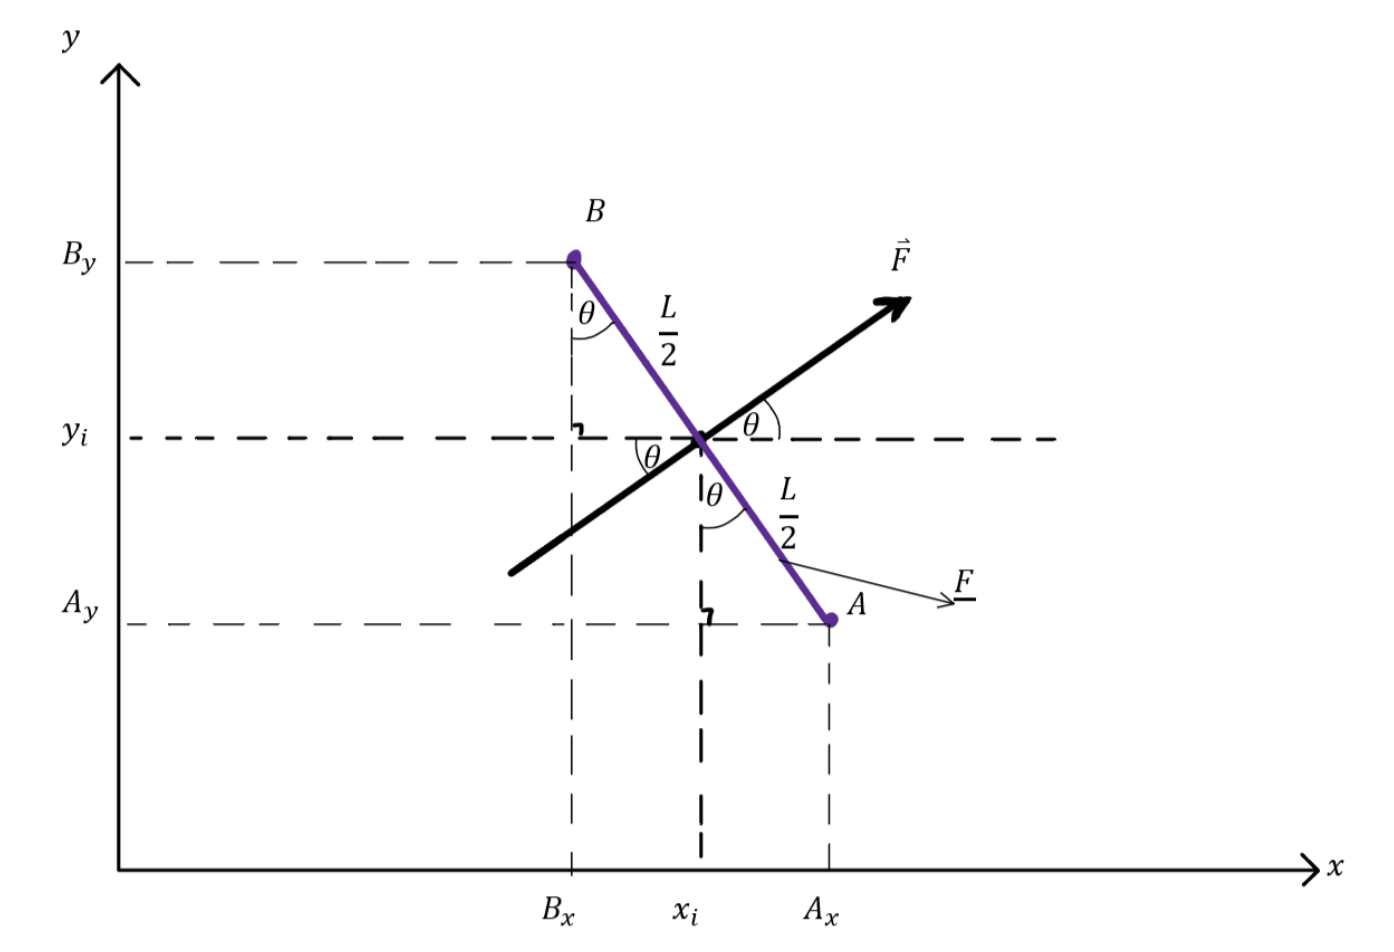
\includegraphics[scale=0.4]{Documentation_images/Geometry of 1 stack sheet}
	\caption{Sketch presenting the Geometrical arguments needed to define stack sheets, based on field magnitude and direction(indicated well by an arrow vector as shown)}
	\label{fig:1 sheet}
\end{figure}
\noindent For \( x_i\) and \( y_i\) marking the $i$\textsuperscript{th}  considered position in the field, with its corresponding angle to the $x$-axis (ccw). Technically, points \(A\) and \(B\) as well as $\theta$ and $\vec F$ depend on the position in space that is considered, therefore, should include the subscript, '\(i \)'. This was not added for figure clarity. \\
The stack, shown in purple, is perpendicular to $\vec F$  with end points $A$ and $B$ separated by distance $L$ (in the code, defined as a fraction of graph scale).\\
From these, through simple geometry, one obtains the following equations:
\begin{equation}
\label{T1} \begin{split}
A_x &= x + \left( \frac{L}{2} \right) \sin( \theta)\,,\\
A_y &= y - \left( \frac{L}{2} \right) \cos( \theta)\,,\\
B_x &= x - \left( \frac{L}{2} \right) \sin( \theta)\,,\\
B_y &= y + \left( \frac{L}{2} \right) \cos( \theta)\,,
\end{split}
\end{equation}
describing the positions of points \(A\) and \(B\) in terms of their Cartesian components.\\
These also function generally as operations that displace a point on the vector in the direction perpendicular to the arrow, by a corresponding length - here by \( \frac{L}{2} \)\,. \\

To then displace the stack sheet by distance $d$ in the direction parallel to the arrow as shown in Figure~\ref{fig:parallel disp.},
\begin{figure}[H]
	\centering
	%\graphicspath{ {c:/Users/macus/Desktop/Uni/summer internships/Moustafa - Differential Forms/images/} }
	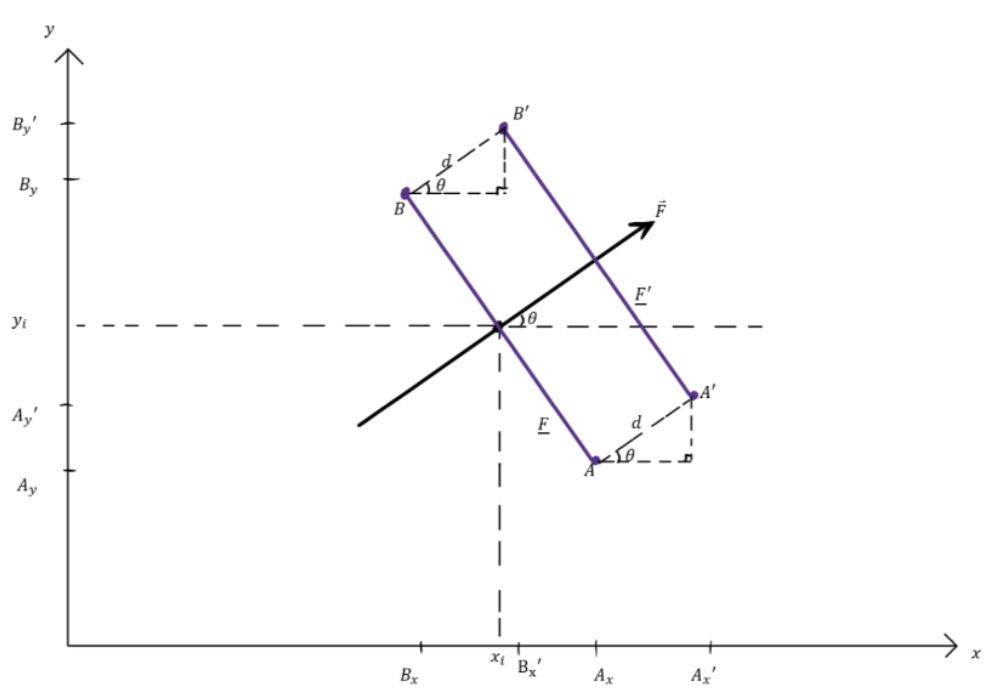
\includegraphics[scale=0.38]{Documentation_images/Geometry of 1 stack sheet, displacement 1}
	\caption{Sketch presenting the geometrical arguments needed to displace stack sheets in the direction parallel to the vector field direction at that point, (again - represented by an arrow)}
	\label{fig:parallel disp.}
\end{figure}
\noindent we use the following translation equations:
\begin{equation}
\label{T2} \begin{split}
A_x' &= A_x + d \cos(\theta)\,, \\
A_y' &= A_y + d \sin(\theta)\,, \\
B_x' &= B_x + d \cos(\theta)\,, \\
B_y' &= B_y + d \sin(\theta)\,, 
\end{split}
\end{equation}
which again function as general operations for such parallel displacements by any distance \( d \), from the centre.\\
To define the arrowhead on that stack vector, both translation operations, eqs. (\ref{T1}, \ref{T2}), need to be used to obatin points to be connected as shown on the figure below

\begin{figure}[H]
	\centering
	%\graphicspath{ {c:/Users/macus/Desktop/Uni/summer internships/Moustafa - Differential Forms/images/} }
	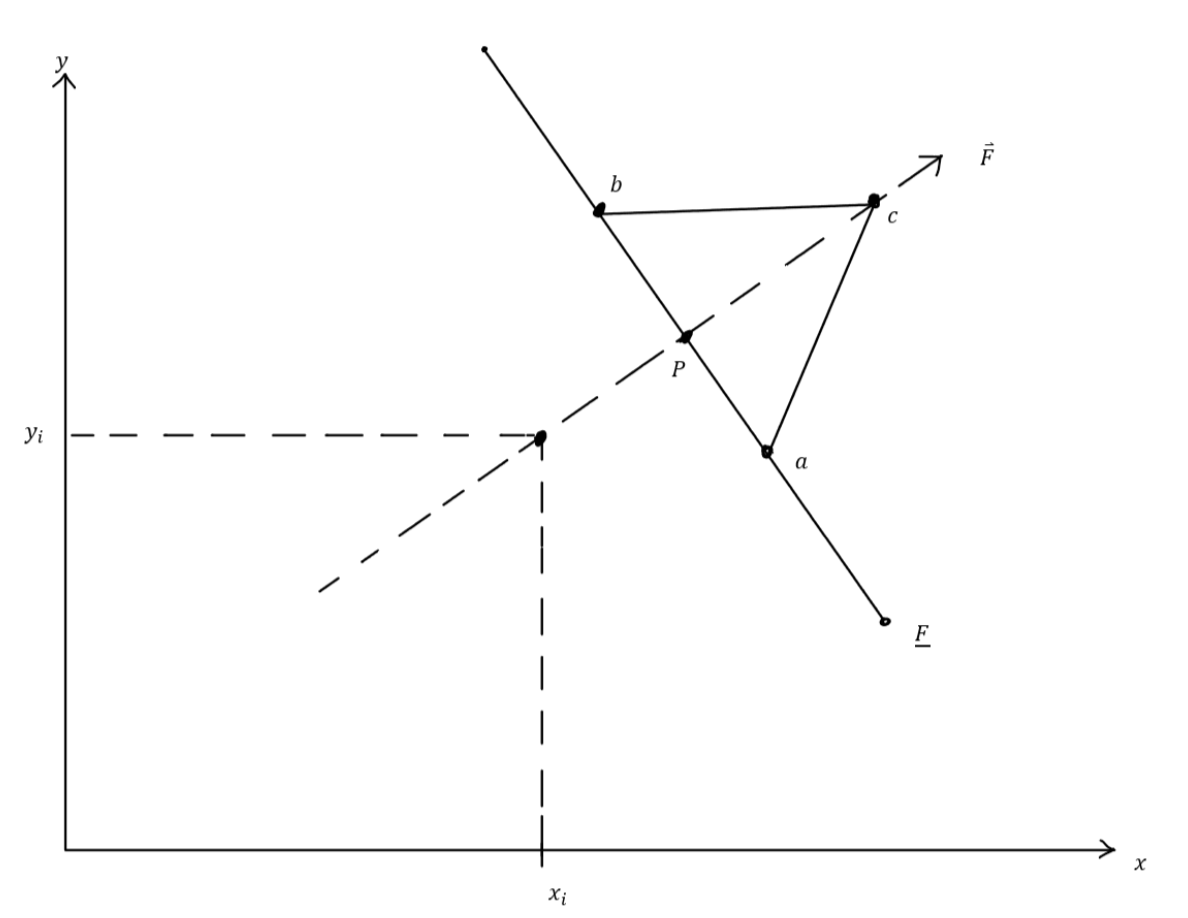
\includegraphics[scale=0.3]{Documentation_images/Geometry of 1 stack sheet, displacement 2}
	\caption{Sketch presenting the geometrical arguments needed to define the arrowhead on each stack vector)}
	\label{fig:arrowhead gometry}
\end{figure}
\begin{align*}
P_i &= \left( x_i + \frac{L_s}{2} \cos( \theta_i) , \  y_i + \frac{L_s}{2} \sin( \theta_i) \right) \\
a_i &= \left( P_{x, i} + \frac{L_s}{w_{head}} \sin( \theta_i) , \  P_{y, i} - \frac{L_s}{w_{head}} \cos( \theta_i) \right)\\
b_i &= \left( P_{x, i} - \frac{L_s}{w_{head}} \sin( \theta_i) , \  P_{y, i} + \frac{L_s}{w_{head}} \cos( \theta_i) \right)\\ 
c_i &= \left( x_i + \frac{L_s}{h_{head}} \cos( \theta_i) , \  y_i + \frac{L_s}{h_{head}} \sin( \theta_i) \right)
\end{align*}
\noindent In these equations, variables are defined as shown on the above figure. \( L_s \) is the maximum thickness of the stack, parallel to the direction of the considered vector field, \( w_{head} \) is the width of the base of the arrowhead that rests on the last stack, and \( h_{head} \) is the height of the arrowhead parallel to the vector field direction.

Note that each has also been assigned a subscript \( i \) which does not appear on the figure. This is only done as these coordinates depend on the point in space that is currently being considered. Also note, that for a single sheet in the stack, the initial displacement from \( (x, \ y )\) to \( P \) must be omitted.

\subsection{General from of stack sheet positions, for any number of sheets}

In the code, it was important to define the displacements of each stack sheet, form the middle position of the arrow vector, at each point in the field. Positioning of sheets depends on the magnitude of the vector field at that point in space. The larger the magnitude, the higher the sheet density. As the spread of the sheets is limited to a pre-defined maximum (on the plot, not physically), this increase in density corresponds to more stack sheets being present.\\
One way of plotting these, such that all sheets are equally-spaced is to consider odd and even number of stacks separately. We define them by displacing stack sheets along the arrow by certain lengths (as per the equations above) from the middle position (the considered position in the field).\\

\noindent For {\bf odd number of stack sheets}, the following pattern was noticed:\\
\small
For 1 sheet: no displacing is needed $\Rightarrow$ $\pm0$\\
For 3 sheets: none, and ends of the stack $\Rightarrow$ $\pm0$ and  $\pm\frac{1}{2}$ $\longrightarrow$ technically $\pm\frac{1}{2}$ $\cdot$ $L_s$\\
For 5 sheets: none, ends, and points equally between $\Rightarrow$ $\pm0$, $\pm\frac{1}{2}$ and $\pm\frac{1}{4}$\\
For 7 sheets: $\Rightarrow$ $\pm0$, $\pm\frac{1}{2}$, $\pm\frac{2}{6}$ and $\pm\frac{1}{6}$ $\longrightarrow$ At this point, note that $\frac{3}{6} = \frac{1}{2}$ (obvious but important)\\
For 9 sheets: $\Rightarrow$ $\pm0$, $\pm\frac{1}{2}$, $\pm\frac{3}{8}$, $\pm\frac{1}{4}$ and $\pm\frac{1}{8}$ $\longrightarrow$ Again, $\frac{1}{4} = \frac{2}{8}$ and $\frac{1}{2} = \frac{4}{8}$\\
For 11 sheets: $\Rightarrow$ $\pm0$, $\pm\frac{1}{2}$, $\pm\frac{4}{10}$, $\pm\frac{3}{10}$, $\pm\frac{2}{10}$  and $\pm\frac{1}{10}$\\
\vdots\\
\normalsize
\noindent These display the following recursion:\\
The displacement along the arrow as a fraction of total stack length $L_s$, of the $s$\textsuperscript{th} sheet, when drawing $n$ stack sheets overall, for odd $n$ is:

\[ \pm{ \frac{s}{ \left( n-1 \right) }}\,, \]

\noindent where we require the fractional displacement (from the middle position) to not exceed half of the total length therefore:\\
\[ 1 < s < \frac{1}{2} \left( n-1 \right)\,.\]\\

\noindent For {\bf even number of stack sheets} this pattern emerges:\\
\small
2 sheets:$\Rightarrow$ $\pm\frac{1}{2}$\\
4 sheets:$\Rightarrow$ $\pm\frac{1}{2}$ and $\pm\frac{1}{6}$\\
6 sheets:$\Rightarrow$ $\pm\frac{1}{2}$, $\pm\frac{3}{10}$ and $\pm\frac{1}{10}$ $\longrightarrow$ Note again that $\frac{1}{2} = \frac{5}{10}$.\\ From here on continue with those not reduced fractions:\\
8 sheets: $\Rightarrow$ $\pm\frac{1}{14}$, $\pm\frac{3}{14}$, $\pm\frac{5}{14}$ and $\pm\frac{7}{14}$\\
10 sheets:  $\Rightarrow$ $\pm\frac{1}{18}$, $\pm\frac{3}{18}$, $\pm\frac{5}{18}$, $\pm\frac{7}{18}$ and $\pm\frac{9}{18}$\\
\vdots\\
\normalsize
These display the following recursion:\\
The displacement along the arrow as a fraction of total stack length of the $s$\textsuperscript{th} sheet, when drawing $n$ stack sheets overall, for even $n$ is:

\[ \pm\frac{2s+1}{2 \left( n-1 \right) }\,, \]

\noindent where we require the fractional displacement to not exceed half of the total length therefore:

\[ 1 < s < \frac{1}{2} \left( n-2 \right)\,. \]

\noindent Alternatively, each can be defined separately, manually, if a small amount of sheets is needed.

\subsection{variables in stack plot code}

This has been implemented in code. The parameters for this are as follows:

\begin{itemize}
	\item $L$ is the length of the positive $x$ and $y$ axes,
	\item pt\textunderscore den is the number of points along each axis,
	\item $a$ is a linear scaling of the field,	
	\item $u$ is the vector field $x-$component, $v$ is the vector field $y-$component $\longrightarrow$  Alternatively: $Fr$ is the radial component and $Ftheta$ is the angular component
	\item orientation is a sting that defines how the arrows pivot,
	\item scale is a linear scale on the quiver plot arrows,
	\item delta is the extra length along the axis to show, past the defined grid, full emerging arrows from border points,
	\item fract is the fraction of graph length equal to stack sheet in direction perpendicular to arrow,
	\item s\textunderscore max is the maximum number of stacks to use,
	\item sheet\textunderscore L is the length of stack perp. to arrow,
	\item s\textunderscore L is the maximum length of stack sheet parallel to arrow,
	\item w\textunderscore head is the width of the arrowhead base as the fraction of the stack sheet length perpendicular to the arrow,
	\item h\textunderscore head is the length of the arrowhead parallel to the arrow, as the fraction of the total stack size parallel to the arrow,

\end{itemize}


\section{Initial GUI of the quiver and stack plot}

\subsection{Explaining user defined functions in the GUI code}

\textbf{parity}: this function takes an input of an integer and returns True ($1$) is it is even and False ($0$) when it is odd. It is useful when defining stack sheets as displacements from the middle position, as the formulas are different for even and odd number of sheets per stack.\\
\textbf{G}: it takes three inputs $\Rightarrow$ $s$: the recursion of sheet displacing from the middle position (which pair is being completed), $n$: how many sheets are to plotted in total and $c$: which is the \textbf{bool} value from the parity function\\
\textbf{stack\textunderscore plot}: takes the following inputs:
\begin{itemize}
	\item $xg$ and $yg$: the grid of points to be used when plotting the field
	\item $ax$: the axis to plot on
	\item $u$ and $v$: the $x-$ and $y-$components of the vector field to be plotted
	\item s\textunderscore max: maximum number of sheets to plot, changes how dense the plot appears
	\item $L$: changes the size of axis (in both x and y equally, from origin)
	\item pt\textunderscore den: defines the number of points on each axis that create the grid
	\item fract: defines the size of the stack sheet (as a square) as a fraction of total graph size
	\item arrows (optional, default=True): Bool variable, defines if arrows should be plotted on top of the stacks (when True), or if only stacks are to be plotted (when False)
	\item orientation (optional, default='mid'): sets the pivoting point of the arrows about that grid point that they are defined at.
	\item scale (optional, default=1): Linearly scales the arrows in the quiver plot
	\item w\textunderscore head (optional, default=8): sets the fraction that defines the width of the arrowhead at its base (on the stack), from the total size of the stack.
	\item h\textunderscore head (optional, default=4): Sets the fraction that defines the height of the arrowhead parallel to the vector field magnitude at that point, from the total size of the stack.
\end{itemize}
\textbf{on\textunderscore key\textunderscore press}: Function that tracks mouse key presses, needed for the 'Matplotlib' toolbar to function\\
\textbf{format\textunderscore eq}: Takes a single string, converts all variables in it that are common in vector field equations, and turns them into things that python can understand. Returns the corrected string
Might be worth noting that many functions are untouched, because, to avoid issues in string replacements in compound function names, we use functions as defined by the numpy library b y importing them directly. This way the user can input their expressions in the standard, consistent, numpy format (without the initial module name calling). \\
\textbf{eq\textunderscore to\textunderscore comps}: Takes the two strings given by the user (equations for the field in the $x$ and $y$ directions) as well as the x and y grids. Uses the above function (format\textunderscore eq) to make the string 'python readable'. If one or more of the strings does not contain $x$ or $y$, it defines an array of ones and multiplies by the given constant. This is done for the component to be over all points along the grid and for shapes to match. Otherwise, it evaluates the given equation and returns the vector field components $u$ and $v$ in the usual way.\\
\textbf{vect\textunderscore type\textunderscore response}: Responds to changes in Radio-buttons that set the type of field to be plotted (arrow, stacks or both). Takes in a value from the Radio-buttons corresponding to the chosen field type. It clear the current plot. Checks which button has been selected and uses ax.quiver and previously user defined stack\textunderscore plot to create the updated graph. It then updates it on the GUI by using canvas.draw() for the canvas being defined on the main window, in its own frame. Returns no variables.\\
\textbf{PLOT\textunderscore response}: Responds to the `PLOT' button being pressed. Updates the axis scaling, point density, maximum number of sheets per stack, linear scaling (`$a$') and the new field components. Takes in no input. collects all needed variables by the `.get()' method of Tkinter objects. After running, it plots the new specified field, with the new parameters as a stack only plot and changes the status of the Radio-buttons to one again be - stacks only (therefore for tensor (same variable name as in VFA java code) to equal 0)\\
\textbf{custom\textunderscore btn\textunderscore response}: when the button called `customise' is pressed, this function responds by opening a new (`optimisation settings') window, in which features can be customised. It includes entry boxes where the user can input new values for parameters such as `fract', `w\textunderscore head' and `h\textunderscore head' (described previously). These are initially filled with current values, changing them and pressing `SUBMIT ALL' updates the plot.\\
\textbf{custom\textunderscore submission}: Responds to the `SUBMIT ALL' in the new `optimisation settings' window. When the button is pressed, the input values are globally saved. The current axis are cleared, a new plot is constructed as per the new specifications and it is displayed on the `canvas' of the correct frame. The updated plot is initially only a stack plot, therefore the radio-buttons are returned to the original position of `stacks'. The new window is then closed.

\section{Mathematically: 2-forms from 1-forms, exterior derivative (on $\mathbb{R}^{m}$)}
The code includes a script that calculates 2-forms from a given 1-form in a specified number of dimensions.
It requires input of the 1-form components respectively to their elemental 1-form (in code: string\textunderscore x, string\textunderscore y, etc.), variable arrays (in code: $x$, $y$ etc.) as well as grids (in code: $xg$, $yg$, etc.) of these and a list of symbols for each variable used in the equations (coords).
The code, so far, has to be changed manually to include the change of all given components from \textbf{string} type to \textbf{sympy.core.mul.Mul}. The number of used dimensions has to also be input as an integer (`$m$' in the code). The variable, `expressions' has to also be appended with the correct number of components.

\noindent Python cycles over the components and the given symbols for variables, differentiating each. To improve efficiency, the derivatives have not been completed when components are to be differentiated with respect to their corresponding elementary 1-form (these go to zero). The results are saved into an (m $\times$ m) array called `ext\textunderscore ds'. The array is of data type `object', as it must store strings of arbitrary length in each of its components. It stores all the found derivatives, with components changing along the rows, and variables changing along the columns.
Each derivative expression is also changed into a string, This is done to append needed prefixes onto them and to later use them with the eval() function, such as brackets and negatives. Minus sings (strings) are then appended to the upper right hand-side of the matrix. This is done to correct for the elementary 2-forms being in the wrong order.

\noindent This, completed, array is then taken through loops that extract the components of each elementary 2-form. These components are symmetrical elements, therefore extracting them includes taking elements with the same $i$ and $j$, switched in the coordinates. A `pair' variable is introduced to keep track of how many times the loop extracted a pair of 2-form components and merged them. As only 2-forms are being calculated, there is always 2 components being extracted toward one elementary 2 form (including zeros as components) The number that this variable reaches is the number of components of a 2 form on $\mathbb{R}^{m}$, which was found to be given by triangular numbers. Resulting pairs are stored in an array of 1 column and a number of rows determined  by the triangular number of dimensionality. This array is called `result', and stores objects (it must consist of strings of varying lengths for each element). Each time a new pair is being considered, the element from `result' is cleared to exclude the initial `NoneType' variable present. When appending the components, it is checked that if one or more of them evaluated to zero, they are not appended.
The result is printed, as a vector, whose rows correspond to different 2-form elements. The order is as follows:
For m=3:
\begin{center}
	\begin{tabular}{c}
		$ dx \wedge dy$, 
		$ dx \wedge dz$, 
		$ dy \wedge dz$.
	\end{tabular}
\end{center}

For m=4 these become:

\begin{center}
	\begin{tabular}{c}
		$ dx \wedge dy$,
		$ dx \wedge dz$,
		$ dy \wedge dz$,
		$ dx \wedge dw$,
		$ dy \wedge dw$,
		$ dz \wedge dw$,
		
	\end{tabular}
\end{center}
etc.

These follow the component pairs as they appear in the lower-right of the matrix (ext\textunderscore ds), in order that follows each line, until the main diagonal.
It can be clearly visualised on the example of the 2-form on $\mathbb{R}^{4}$ as follows:
\begin{equation}
		\begin{pmatrix}
			0 & dy \wedge dx & dz \wedge dx & dw \wedge dx \\
			dx \wedge dy & 0 & dz \wedge dy & dw \wedge dy \\
			dx \wedge dz & dy \wedge dz & 0 & dw \wedge dz \\
			dx \wedge dw & dy \wedge dw & dz \wedge dw & 0 \\
		\end{pmatrix}
\end{equation}

Each component of the outcome (`result') is then formatted in such a way as to be understood by python's eval() function and the evaluation of each is saved into a variable called `form\textunderscore 2'. This has to be composed of m dimensional arrays, one for each elemental 2-form component (given by the triangular numbers from the used dimensions `m').

\begin{center}
	\Large
	IMPORTANT - CONVENTION\\
	\normalsize
	There exists a convention on $\mathbb{R}^{3}$ which allows for simple matching of 2-forms to unit vectors used in vector calculus. By this convention, the elemental 2 forms used are not as stated above ($ dx \wedge dy$, $ dx \wedge dz$, $ dy \wedge dz$), but instead, are given by: $dx \wedge dy$, $ dz \wedge dx$, $ dy \wedge dz$. This allows for use of the standard Cartesian coordinates with the simple rule that the 2 forms correspond to unit vectors. This convention was not followed in this code, as it is irrational to use it in $m>3$, and it was established that it shadows an important aspect of differential forms. Wedge products are not defined in extra dimensions (in a way that a curl is defined in a direction the filed does not occupy, perpendicular to it). Wedge products have their orientation defined through the axial sense (clockwise and counter-clockwise). This means that their wedge product does not occupy extra dimensions. This can only be clearly retained, as used in higher dimensions, when the convention on $\mathbb{R}^{3}$ is abandoned. This is exactly what is done in the code. This code gives the 2 forms defined through clockwise (negative) and counter-clockwise (positive) orientations.
\end{center}

\section{Inset Plots}
\subsection{Derivative Window}
Selecting the `Derivative Plot' radiobutton (top right frame) allows the user to display a small grid showing the local derivative of the field by clicking the vector field (top left frame) at the point of interest. The derivative field plots according to the 'tensor' variable (i.e. if the vector field is currently plotting with stacks/arrows, the derivative field will also.)

The radiobutton variable `click\textunderscore option' is a tk IntVar and is converted to an integer in the response function `click\textunderscore option\textunderscore handler'. `click\textunderscore option' is then used to determine the required click control in the function `on\textunderscore key\textunderscore press': if the `Derivative Plot' radiobutton is selected, clicking calls `deriv\textunderscore calc' which creates the plots. The feature is disabled by selecting the `Tools' radiobutton (`Tools' option refers to the improved functionality of the matplotlib toolbar i.e. for zooming or panning.) \textit{Note: this method still needs work as the toolbar tools still function when `Tools' is not selected.}

The `deriv\textunderscore calc' function takes the $x$, $y$ data click coordinates, the pixel click coordinates to create an inset axis (`deriv\textunderscore inset\textunderscore ax') centred at the user's selected point. The parameters which determine the axis properties are:
\begin{itemize}
	\item dpd: point density of the derivative plot (user sets via drop down menu)
	\item d\textunderscore length: size of the inset axis (user sets via drop down menu)
	\item d\textunderscore range: x and y distance from the chosen plot point over which the derivative is taken (user varies using zoom slider)
	\item d\textunderscore scale: scaling of the arrows in the derivative plot (user varies using zoom slider)
\end{itemize}

The plot is generated by creating new $x$ and $y$ meshgrids (dxg, dyg) with centres at the click data point. Previously mentioned `eq\textunderscore to\textunderscore comps' is then called with the user defined components `string\textunderscore x' and `string\textunderscore y' to generate a local field `u1' and `v1'. The derivative is taken by subtracting the components of the central grid element from every element in the array, leaving du1 and dv1. The 'if' statement checks whether to plot with arrows/stacks/both. To plot the stacks, the `stack\textunderscore plot' function is called with changed input grids and axis to plot based on the internal parameters of the inset plot. The if/continue statement is entered this time, to prevent stacks plotting at the central grid position (as the derivative field is always zero there). Finally, the inset axis is displayed on the canvas using `canvas.draw'. 

\subsection{Zoom Window and Zoom Slider}
The zoom window plots the local vector field components 'u1' and 'v1' on the 'dxg' and 'dyg' meshgrid arrays, in the same fashion as for the derivative. The zoom slider value is used in 'deriv\textunderscore calc' to decrease 'd\textunderscore range' and increase 'd\textunderscore scale' such that the plot shown takes vectors from a much smaller region of the field and makes sure they are sized appropriately. The effect of this can be seen when zooming in on a region of the plot sufficiently, such that a constant field is displayed. As for the derivative feature, low magnifications no longer produce a viable representation of the derivative field, but upon zooming the user can see the derivative field emerge (which tends to a linear field at high magnification). 

\subsection{Divergence and Curl Windows}
The divergence and curl plots are generated using an analytical method. The 'jacobian' function takes the string component entries from the entry boxes in the 'Field Input Frame' and calculates the Jacobian matrix using sympy partial differentiation. The resulting matrix is evaluated at the click coordinates (x\textunderscore m, y\textunderscore m) giving:

\begin{equation}
	J =
	\begin{pmatrix}
		\frac{\partial u}{\partial x} & \frac{\partial u}{\partial y} \\
		\frac{\partial v}{\partial x} & \frac{\partial v}{\partial y} \\
	\end{pmatrix}
	_{(x_m,y_m)}
\end{equation}

For these plots, the 'dxg' and 'dyg' meshgrids must be centred on zero, rather than on the click coords used for the deriv and zoom plots (the first if statement in 'deriv\textunderscore calc' accounts for this.) The component equations of the divergence and curl fields are then calculated:

\begin{equation}
	u_{div} = \left( \frac{\partial u}{\partial x} + \frac{\partial v}{\partial y} \right)_{(x_m,y_m)} \Delta x \quad
	v_{div} = \left( \frac{\partial u}{\partial x} + \frac{\partial v}{\partial y} \right)_{(x_m,y_m)} \Delta y	
\end{equation}
\begin{equation}
	u_{curl} = \left( \frac{\partial u}{\partial y} - \frac{\partial v}{\partial x} \right)_{(x_m,y_m)} \Delta y \quad
	v_{curl} = - \left( \frac{\partial u}{\partial y} - \frac{\partial v}{\partial x} \right)_{(x_m,y_m)} \Delta x
\end{equation}

In this notation, $\Delta x$ and $\Delta y$ represent displacements within the inset axis. As a result, positive curl is shown by a linear field with counter-clockwise flow and negative by a clockwise flow, as would be given by the right hand rule. Additionally, the divergence and curl plots use scaling that matches the field, which ensures that the magnitude of the vectors varies appropriately. 

\section{Line Integrals}
\subsection{Lines}

Upon selecting the 'line integrals' tab, with the polygons drop down selection, the user can draw lines on the plot by clicking to mark the successive start and end points as required. The users click coordinates are stored in a list (LI\textunderscore coord). The function 'line\textunderscore int\textunderscore poly' takes the two most recent entries in the list of coordinates and finds the approximate line integral using the following method:

\begin{itemize}
	\item Small displacements along the line in the $x$ and $y$ directions are calculated based on the last two entries in LI\textunderscore coord (coords of points $a$ and $b$) and the chosen number of intervals along the line, $N$. $dx = \frac{1}{N} (b_x - a_x)$,  $dy = \frac{1}{N} (b_y - a_y)$
	\item A 2xN array 'intervals' is created and stores the coordinates of the points along the line which will be used in the final calculation. This is achieved using a for loop; $intervals(x_k) = a_x + k dx$, $intervals(y_k) = a_y + k dy$
	\item Next the vector field components must be evaluated at each of the interval points along the line. These components are stored in the 2xN array 'uv\textunderscore store'. 
	\item The line integral is approximated by summing the products of the small displacements $dx$ and $dy$ with the respective vector field components at each interval point. Since the displacements are the same along the straight line, the sum is simplified to:
\end{itemize}

\begin{equation}
	\int_{a}^{b} \vec{F} \cdot \vec{dl} \approx \sum_{k=0}^{N-1} \vec{F}(x_k,y_k) \cdot \vec{dl}(x_k,y_k) = dx \sum_{k=0}^{N-1} F_x(x_k,y_k) + dy \sum_{k=0}^{N-1} F_y(x_k,y_k)
\end{equation}

Here, $\vec{F} = F_x \ \hat{i} + F_y \ \hat{j}$, $\vec{dl} = dx \ \hat{i} + dy \ \hat{j}$ and $(x_k,y_k)$ denotes the coordinates of the $k^{th}$ interval point along the line. Each successive line integral is added to the total and displayed in a GUI label. The reset button clears the plot, the list of coordinates and the total, allowing the user to start from scratch.

\noindent This function operates not only over single starlight lines but also joins them head-to-tail to create polygonal shapes by accessing previous mouse click coordinates from LI\textunderscore coord. The polygons can be closed by clicking near \textbf{any} previously clicked point. This is coded by defining these coordinates as equal when the distance between them is smaller than a selected interval 'ctol'. Which is set to be 0.1 (in axis units).

\noindent This function also plots a square grid to aid the user in drawing rectangles on the plot, without the need for an additional function to draw squares. This grid is removed when any other option is selected. 

\subsection{Circles}

Selecting the circles drop down option will allow the user to plot circles on the vector field, updating the position and radius (user selected by entry box) upon every click. Circles are centred on click location. The user is also allowed to select the orientation of the integral by use of a button. This button displays the currently used orientation, and changes when it is clicked (between 'cw' and 'ccw'). To redo the calculation with the newly selected orientation, the plot has to once again be clicked.

The main difference from the calculation of straight line integrals is that the displacement vectors are no longer constant, as they will be tangent to the circle at each interval point. The method is as follows: 

\begin{itemize}
	\item Define the small displacements $dx$ and $dy$ (arrays) for the $N$ interval points using $dx_k = -Asin(kdt)$ and $dy_k = Acos(kdt)$ (changed to negations using an if-else statement, depending on chosen orientation). $dt$ is a small angle increment and is stored as an array in the code (linspace from 0 to 2$\pi$ with $N$ points.) $A$, the magnitude of the displacement vector is chosen to be the length of the circumference swept out by each angle increment, $A = \frac{2\pi R}{N}$. 
	\item Calculate the coordinates of interval points: $intervals(x_k) = x_m + Acos(kdt)$, $intervals(y_k) = y_m + Asin(kdt)$. $(x_m,y_m)$ are the coordinates of the users click. 
	\item Evaluate the vector components at each interval point as before.
	\item Find the total line integral using:
\end{itemize}

\begin{equation}
	\ointctrclockwise \vec{F} \cdot \vec{dl} \approx \sum_{k=0}^{N-1} F_x(x_k,y_k)dx_k + \sum_{k=0}^{N-1} F_y(x_k,y_k)dy_k
\end{equation}



\section{Non-unique and wrong graphical representations of 2 forms on $\mathbb{R}^{2}$}
\subsection{Blocks and stacks}
Two alternative ways of representing 2 forms have initially been considered. Both of which were later established to be incorrect. These are still discussed here, for record and, as it is believed to give good insight into problems that arise when attempting this task 
The first, simpler method considers the 2 form magnitude at different points in space and represents them as squares, whose size is determined by the magnitude, and whose colour shows the orientation, obtained by the sign of the 2 form at that point. This method has been dubbed as plotting 2 forms through 'Blocks'.

\noindent The plotting of these is completed by defining rectangular patches, provided by the matplotlib library. The size of each rectangle is defined in terms of a fraction of a user defined total (customisable) and depends on the relative, unitary magnitude of the 2 form, with respect to its maximum value over the defined region.

\noindent Due to the simple approach of this method, no coding complications occur. The 2 forms are simply represented. However, they do not clearly show the most important characteristics of 2 forms. They, by requirement: have gaps between them, will overlap if magnitudes are large enough and in no way graphically represent the idea of 2 forms being elemental areas through which integration can be completed.\\

A graphically clearer way of representing 2 forms is through the superposition of stacks from elemental one forms. This process includes finding expressions for fields in the $x$ and in the $y$ directions such that the desired 2 form is being represented. These are then plotted using the $x$ field for stacks in the $x$ direction and the $y$ field for stacks only in the $y$ direction.

\noindent The result forms a gird that covers the defined region with squares, whose inside is dissected into further sections (separately in the x and in the y directions), depending on the 2 form magnitude at that position. More dissections occur inside, depending on which component of the 2 form is dominant at that position. This dominating is defined through the expressions of 1 forms that are being superposed.

This approach clearly presents all characteristics of 2 forms. The region is covered, no overlap is allowed and it can be seen how integration over such areas can yield known results. Another characteristic which, through this, can be reproduced is merging of 2 form 'tubes' on $\mathbb{R}^{3}$, which we will return to later.

However, there exist major issues with this approach (which will also be explained in more detail in the coming subsections). These include the above-mentioned processes of finding 1 forms that reproduce the desired 2 form. This has been attempted through two approaches, un-doing the exterior derivative, or through undoing a wedge product. Both of which give the desired 2 form in terms of component 1 forms.


\subsection{2 forms on R2 through the exterior derivative}
One way to obtain a 2 form from component 1 forms is to ask the user for a 1 form and compute the exterior derivative of it. This way, both are known, the 2 form and the 1 form that it originated from. To complete the above mentioned process, the input 1 forms can be differentiated (as in the Jacobian) and the skew-symmetric parts can be taken (these are the components that form the resulting 2 form). These components can then be plotted as stacks in the $x$ direction (differential of the $dx$ component w.r.t $y$) and in the $y$ direction (differential of the $dy$ component w.r.t $x$). However, there exists a problem with this procedure, and that is, the non-uniqueness of the result. Many 1 forms may become the same 2 form upon the exterior derivative, due to cancellations occurring between $dx \wedge dy$ and $dy\wedge dx$ components. This means that, the graphical representation of a given 2 form will vary, depending on its origin. Which should clearly not be the case, as the 2 form should be its own, separate, object, defined uniquely in space.
The cancellations could be solved if code was written that would scan the two resulting equations for any cancelling or merging components and delete or distribute them (respectively). This would be difficult and is not needed. This is because this process will still make the 2 form not unique, it will simply be another representation. There also exists a much simpler method, which we will come back to.

A method of excluding such cancellations was found and implemented such that given 2 forms yield identical representations. This was done through, first obtaining the mathematical expression of the 2 form through the exterior derivative as described previously. The result was then simplified by changing it to a 'SymPy' expression and using the 'simplify' function. Once this was completed, the 2 form was split into two, equal elements, $dx \wedge dy$ and $dy\wedge dx$. Which determine the derivatives of 1 form components that can be used to plot stacks as described previously.
Once again however, this was established not to be fully functional. The issue now was, the splitting of the 2 form is also not unique, it is arbitrary. Any splitting will work, so long as the components return the same 2 form when merged (by inverting the elementary 2 form and adding).

This issue was found to be fundamental. As clear and intuitive as this method seems to be for graphically representing 2 forms, it does not provide a unique way of doing so. In fact, all the representations it does provide are elements of a rotation group ($SO(2)$) of the resulting 2 form. To present this idea more clearly, lets look at the more rigorous proof of the above stated non-uniqueness which arises through splitting the 2 form.

\subsection{Proof of the non-uniqueness of 2 forms}





\subsection{2 forms on R2 through the wedge product}
There exists yet another way of defining 2 forms through stacks that represent 1 forms. This includes splitting the 2 form into components, not into $\wedge dy$ and $dy\wedge dx$ that are understood to originate from the exterior derivative, but into $f(x, y)dx \wedge g(x, y)dy$, where the 2 form is $f(x,y)g(x,y) dx\wedge dy$. This yields another issue. Similarly to the last considered method, the splitting of the 2 form into a product of two functions is not unique. Again, as above for the previous method, it is also possible here to let the user input two 1 forms to wedge together into a 2 form, but once again, this may also include cancellations or merges between components, which make the 2 form not unique.

\subsection{initial 2 form representation as stacks in code}
Due to the fact that unique representations could not be deduced. The code we produced initially allowed the user to choose, what representation they would like to see.

\textbf{User-supplied 2 forms} were being plotted as stacks by splitting the expression into two components $dx\wedge dy$ and $dy\wedge dx$. The splitting of the expression was set by the user via the 'set splitting' button (by default splitting occurs into two equal halves). These have then been plotted as previously stated, one as the $x$ component and the other as the $y$ component. This plotting was done via a function ('form\textunderscore 2\textunderscore components\textunderscore plot') which is very similar in operation to stack\textunderscore plot. The new function however, also uses the end 2 form expression, evaluates it numerically, finds its sign and depending on this, colours the stacks (it is still used in the end version of the code). It was chosen to colour via the convention that grey signifies zero magnitude at that position, red represents positive (axially ccw) 2 form magnitude and blue stands for negative (axially cw) magnitude. Because 2 form areas must fill space, this function includes a variable that sets the minimum number of stacks ('s\textunderscore min') to two. This way, full squares are always being displayed and then dissected depending on magnitude, but will not become open areas. Also, to avoid the same issue, the size of stacks (initially set by the user as a customisation option) is now calculated from the chosen number of points along each axis automatically to fill space (this occurs when tabs are opened and when the number of points is changed). The equation by which this is done is the following:

\begin{equation}
	\label{T2} \begin{split}
		d = \frac{2}{n-1}
	\end{split}
\end{equation}

for the stack size $d$ and the number of points along the axis $n$. 


\textbf{2 forms from the exterior derivative} were plotted by a similar process as above, with the initial addition of finding the mathematical expression of the 2 form and simplifying it (as has been described above) by the find\textunderscore 2\textunderscore form function. Once the 2 form was found, it was input into the entry box for 2 forms and was highlighted in light green to show what is currently being displayed (as opposed to other options including the supplied 1 forms). This process of highlighting is still used in the end resulting code. 


\textbf{2 forms through the wedge product} is (same as in the end resulting code) completed by first asking the user to input two 1 forms that are to be wedged together, in terms of their components in $dx$ and $dy$ (other on $\mathbb{R}^{3}$). This is done by displaying a new window for these inputs after the 'wedge' button is pressed. Once these are submitted this extra window is closed, although its entries are saved and display again when it is re-opened. The inputs are simplified by briefly passing them into 'SymPy' expressions. The components of these inputs were then calculated using the previously described 'eq\textunderscore to\textunderscore comps'. The 2 form was found by concatenating strings of input in such a way as to result in the correct 2 form. This was also simplified in the same way and displayed in the 2 form entry box, which, once again, light up to a light green. The plotting of superposing stacks was then completed by using the stack\textunderscore plot function with disabled arrowheads.

Mathematically, given $w_{1} = f(x, y) dx + g(x, y) dy$  and $w_{2} = h(x, y) dx + m(x, y) dy$. The 2 form on $\mathbb{R}^{2}$, $\alpha$, must be made up of:


\begin{equation}
	\label{T2} \begin{split}
		\alpha = w_{1}\wedge w_{2} = f(x, y) dx\wedge m(x, y) dy + &h(x, y) dy\wedge g(x, y) dx \\
		= \\
		f(x, y)m(x, y) dx\wedge dy + h(x, y)g(x, y) dx\wedge dy &= (f(x, y)m(x, y) - g(x, y)h(x, y)) dx\wedge dy  
	\end{split}
\end{equation}


which is used to be found by and plotted as stacks when an if condition was satisfied, stating that none of the entries were zero. Currently, this is still being used, to find the 2 form mathematically.
Two rectangular stacks with the scaling factor were accounted to by giving similar colours to the vertical  and horizontal stacks (red and green). After the first rectangular stacks were added the second group either sat on top of the first (in which case scaling contribution was zero) or sat in some gaps, hence increasing the density as result of its scaling function.
If any of the coefficient functions (f, g, h or m) were zero, the stacking reduced to one function together with its elemental 2 form $dx\wedge dy$, these were executed in the 'elif' options under the if statement. This code, although it did not use splitting, and included cancellations was also incorrect. This was because, the 2 form did not fill space, its x and y contributions were implied by density of long vertical and horizontal lines that span many stacks etc.


\subsection{2 form representation as blocks in code}
The simpler method was also implemented to show the comparison between the  locally detailed, non-unique (stacks) and locally undefined, global, unique (blocks). Despite the fact that blocks were known to be the wrong representation, an option to plot them was still implemented to highlight the difference between unique and non-unique representation methods. 
This was more simply implemented by defining the above described process of plotting blocks in a single function and calling it with the appropriate 2 form whenever necessary.
The option as to which should be used was given to the user through radio buttons, however, when stacks was selected, a message box displayed, warning the user of the non-uniqueness of the result and its dependancy of their splitting choice.

\section{Correct 2 form on $\mathbb{R}^{2}$ representation}
A unique, locally detailed, space filling representation of 2 forms has been found. This is the representation currently used by the code. It continues the idea of representing 2 forms as superposition of stacks, however, no longer as a superposition of two separate 1 forms. The way it is currently done is through plotting the 2 form expression as stacks in both $x$ and in $y$ separately. This is equivalent to equally splitting the 2 form in the previous representation, however, it was found that, despite being only one element of the $SO(2)$ rotation group, it is sufficient to describe all 2 form properties. Thus it was established that this representation is fulfilling.

The reason for that statement is the following. The 2 form, to be correctly represented must contain information about oriented areas, and how their number varies in space. It was originally thought that the information about such variation must be included in the dominant component ($x$ or $y$ of the 2 form, at that position). However, this can also be more simply represented by looking at variation in the number of areas at neighbouring positions.

The current method of plotting relies on constructing a space filling, square gird and dissecting each square (equally in the $x$ and $y$) depending on the 2 form magnitude at that position. This guarantees uniqueness as the magnitude is well defined, and it continues to display the variation, when the grid is fine enough and s\textunderscore max value is chosen to be sufficient.
The splitting ambiguity can be thought of as confusion by attempting to split these squares not by the 2 form alone, but by considering extra information - dominance of the $dx$ or $dy$ component. This information is not contained in the resulting 2 form, and therefore, of-course it cannot be reliably, clearly represented.
The problem can (on some level) be compared to being given an area to draw (the 2 form) and saying that this cannot be done because the shape was not given (1 forms). Yes, the shape will not be known, but it is arbitrary and is not contained in the asked task (of drawing an area, the 2 form). In this analogy, our method can be compared to responding to such a task by drawing many small squares whose total area matches that given area. The task has been accomplished, and it can easily be seen how these can distribute over space to different shapes. We draw squares, not rectangles in $x$ and $y$, but the variation over these can easily be seen by the number of these squares over the region changing.

It may also be noted that this idea was sparked by the problem of cancellations, which was found to be the case of correct arithmetic, but incorrect geometry. Mathematically, the components will cancel to give the same 2 form, however, when attempting to display the 2 form in terms of 1 forms this cancellation will not be geometrically valid.
Hence, the 2 form can always (mathematically) be found as two 1 forms, however, to represent it graphically, we must abandon this approach. Surely it is correct, but it is not necessary to represent 2 forms. All that is needed is the 2 form itself.

This has been implemented by simply removing options to plot blocks and to choose splitting factors, instead, the 2 form was simply plotted by the same function as previously, half in the $u$ and half in the $v$.

\section{Other calculus using 2 forms}
\subsection{Interior derivative acting on 2 forms}
The code includes the option to calculate the interior derivative of a 2 form (and a 1 form) on $\mathbb{R}^{2}$. \textit{Note: it has not yet been generalised to $\mathbb{R}^{3}$}. After pressing the button ('interior derivative'), a new window displays, which asks the user to chose which option to evaluate with. The interior derivative can be applied to a 2 form only, or to a 2 form and 1 from simultaneously. Once the option is chosen, it asks the user for a vector field to do the calculation with respect to in terms of the $x$ and $y$ components. The two windows are then shut.

\noindent \textbf{To complete the interior derivative of the 2 form}, the code takes given inputs (2 form and 'background' vector field), formats and simplifies them (as before) and calculates the resulting 1 form by the standard procedure (thanks to linearity of the interior derivative):

\begin{equation}
	\label{T2} \begin{split}
		\iota_{\vec{u}}(\omega) = f u_{1} dy - f u_{2} dx
	\end{split}
\end{equation}
where $\omega = f dx\wedge dy$ and $\vec{u} = u_{1}dx + u_{2}dy$.
This is found numerically and as a string, to be able to plot it, and to be able to display it to the user.
This resulting 1 form in put into entries for 1 form components and the boxes are coloured into light green to show that these are currently displayed. The result is plotted using the 'form\textunderscore 2\textunderscore components\textunderscore plot' function with $u$ and $v$ given by the expression as shown above. This function is used as opposed to stack\textunderscore plot, as it also includes colouring of stacks, depending on the sign of the original 2 form at that location.
This process is specified in the 'Int\textunderscore deriv\textunderscore 2\textunderscore form' function. This is called when the selected option is '2 form only' by the 'Int\textunderscore deriv\textunderscore 22\textunderscore form' function.

\noindent \textbf{To complete the interior derivative of the 2 form and the 1 form} a similar process is completed, but the 1 form is also taken into account. The 1 form calculation is completed by a function called 'Int\textunderscore deriv\textunderscore 1\textunderscore form'. The two functions are separate in order to be able to more easily call their combinations when user wished to use both, or each one separately. This function completes a similar process to the above described (for 2 froms) however, it is based on a different equation, as follows:

\begin{equation}
	\label{T2} \begin{split}
		\iota_{\vec{u}}(\omega) = f_{x} u_{1} + f_{y} u_{2}
	\end{split}
\end{equation}
where $\omega = f_{x} dx + f_{y} dy$ and $\vec{u}$ is as previously. The result is a zero form (scalar function), which can be most easily represented via its contours. Because in the GUI, there exists no entry box for a zero from, the result of that is displayed underneath the 1 form entry box in red, as a Tkinter label.

When \textbf{the two require being computed together}, both function are called with appropriate canvas preparation by the function 'Int\textunderscore deriv\textunderscore 21\textunderscore form'. This finds the result of the 2 form, which returns a vector field, which 'sits on top of' the computed 1 form. This can visualised as a vector field lying on a scalar function landscape.

\noindent These functions are called by a response to the PLOT button in the window where the user defines the background vector field. Depending on which option was selected in the previous window ('2 form only' or 'both'), The plot button binds to different functions and hence responds appropriately.

\subsection{Hodge}


NOT IMPLEMENTED YET



\section{Forms on $\mathbb{R}^{3}$}
\subsection{Representing 2 forms on $\mathbb{R}^{3}$}
On $\mathbb{R}^{3}$, 1 forms are parallel, two dimensional sheets, perpendicular to the elemental 1 form. 2 forms can thus be represented as intersections of such sheets, forming tubes, which define elemental, oriented areas that are the 2 form. This is very difficult to show on a solid, rotating gird of many, small intersecting sheets, therefore a different approach has been used. The code lets the user inspect planes though a three dimensional cube by selecting the viewing axis and the depth into the solid.
This, visually, gives the same looking 2 forms. This is because the viewer is slicing through the tubes at a selected height.

As the sheets are defined by stacks which run perpendicular to their corresponding direction, if any component of the viewed 2 form was in the direction of the axis along which the viewer is looking, the tubes would not be pointing in their direction and thus would be closed. Therefore:
\begin{itemize}
	\item Viewing from the $z$ axis, only the 2 form components in $dx\wedge dy$ would be apparent
	\item Viewing from the $y$ axis, only the 2 form components in $dx\wedge dz$ would be apparent
	\item Viewing from the $x$ axis, only the 2 form components in $dy\wedge dz$ would be apparent
\end{itemize} 

The process of calculating and plotting these is similar to the previously defined process used in plotting two forms on $\mathbb{R}^{2}$ (the new, corrected one). The initial methods for representing 2 forms (blocks and 1 form splitting) have initially also been implemented here, but have since been changed to correctly display.

This time the 'result' calculated by the two form finder (described previously) has three entries, each of which needs to be split into two equal parts (again, used to be customisable by the user, to display non-uniqueness when represented using split 1 forms. That process used six components (two for each plane) calculated from the found 2 form, which were plotted as stacks. Only three of which are now needed because the new representation is identical to equal splitting, however, the six were kept in the code. This is because that allows us to still use the eq\textunderscore to\textunderscore comps function, which always works with two inputs. These are then plotted similarly to the process of doing so on $\mathbb{R}^{2}$. It is done by a function (form\textunderscore 2\textunderscore components\textunderscore plot\textunderscore 3), nearly identical to the one used on $\mathbb{R}^{2}$, with the change that this one accepts all parameters in three dimensional grids and splits them correctly to corresponding planes, which is completed through slicing.
This slicing is done an if-elif-else statement, one test for each axis projection. These deal with slicing grids, stack components and the slicing of the 2 form signs array.
The strange thing about this slicing is that, due to the way meshgrids are defined ; while the component along the z axis is in fact a slice of $[:, :, height]$ as expected. The x and y slicing is switched.
Also, singularities now not only must be excluded in the components (or in the magnitude) but also when the 2 form sign is to be taken.
It may also be noted that this function, as the corresponding one on $\mathbb{R}^{2}$, also has (for the same reason) s\textunderscore max set to two.

\noindent An extra process is required to make tubes update in the viewing axis accordingly to changing the height along it. This is because when expressions are proportional to functions of the viewing axis coordinate, they would not scale, they would simply be an additional constant that would vanish in the representation because of our applied relative scaling of stacks. A global scaling needs to be applied to correctly handle this.
This is done by finding the maximum value across all height points (excluding singularities), defined globally, for that two form component, dividing the local maximum (in the plane) by that global maximum and multiplying the relative scaling array by that value.

It may be worth noting that a slider has not been implemented to complete the process of changing the viewing height along the viewing axis. This was  due to issues with Tkinter sliders, in getting them to go up in any, user defined intervals (without rounding, as then the exact value has to be found in the array to obtain its index for slicing).

\section{Singularities}
It was noticed when experimenting with the Vector Field Analyser \url{https://math.la.asu.edu/~kawski/vfa2/index.html} that singularities in fields break the code. Worst of all, singularities that fall on or near grid points, break the linear scaling, making the entirety of it plot as a zero field (relatively). Not only that but singularities were not displaying when off the grid, and undefined regions were simply not plotted. We have decided to input such options into our code.

To begin with, there are some issues with the ideal scenario of finding all singularities, plotting them on and excluding them from scaling. However, this is difficult mainly due to the fact that no function has been found that will record singularities in mathematical expressions above $\mathbb{R}^{2}$. Only SymPy 'singularities has been found' which functions for single variables functions and has inconvenient outputs (for plotting).

Many attempts were made to include such in our code, with limited success.
The end result includes a three way mechanism for coping with singularities.
First of all, if any such points (including not a number evaluations, infinities and values above $1e15$ that python at times mistakes for infinities) lie on a grid point, they are removed and plotted on. If the value was large, or infinite (according to python evaluation), it is plotted as a red circle. If it was evaluated as NaN, it is plotted as a grey square.
If singularities lie off grid points, two options are given to the user. They can search through the region with a finer grid of a chosen number of points per side, or define their own singularity.

If they choose to search, the code runs through a grid of finer points (as specified) looking for on grid large values (above $1000$), or infinities and plotting them as described above (but smaller). The mechanism for doing to is made for efficient by not saving all points to evaluate at, however, it can still be very slow for very fine grids, therefore the user is warned of slow processing if the value they input is above $200$ per axis.

If they choose to define their own singularities. They can do so by defining an equation in $x$, an equation in $x$ or by supplying point coordinates. This will plot the given equation on the graph. These plots will stack if more than one is given. Many expressions can also be input simultaneously by separating them with a semi-colon (';'). If the expression in $y$ is input in terms of $y$ only (or conversely the $x$ expression is in terms of $x$ only), it is assumed to be and error and is plotted as if the opposing variables was given. For example, inputting $x = \sqrt{4 - x^2}$, instead of solving the equation for x , a line of $x = \sqrt{4 - y^2}$ is plotted.

The point option accepts points in standard format ($x$ coordinate, then $y$), separated by a comma. If more than one is to be input, it can be done through a semi-colon as before. The code does not accept brackets surrounding the point coordinates.

These self input singularities also run a background check. When an expression or a point singularity is input, the code will check for singular points along it. If it does not find any (not even a single point), it will warn the user that the code could not find any singularity at their asked positioning. Perhaps it is worthy of note that, despite such warning being showed, as asked, the plot will be created. It is also important to note that the code will not display this, even if most points evaluate not to be singular. This has been implemented because evaluations are not very exact and can at times be faulty.

\end{document}